\chapter{Website}
\section{Features}
In this project, the only objective of the website was to collect information from the user, and stock them in the database.

When an user comes for the first time on the website, he has to sign up and provides some informations about the company. After this operation, the user can access to his control panel where he can:
\begin{itemize}  
\item Create or edit his switchboards.
\item Manage operators\footnotemark.
\item Manage the company's informations
\end{itemize}  


\footnotetext{Operators are people who will receive calls from the switchboard.}

\section{Available modules}

\subsubsection{Playback}

\subsubsection{Operator}

\subsubsection{Queue}
\subsubsection{User input}



\section{Overview}
In this project, the website had to be the only way to interact with the server. Through a simplified website, the users have to fill required informations, then they are saved into a database.
\newline

The website is based on \textbf{Spring} technology,  it follows the MVC convention (\textit{Model-View-Controller}). Each layer has its own role in this convention.


\begin{itemize}  
\item The views represents the content the users will be able to see. In our implementation, these files contains special HTML and special tags to allow dynamic contents. 
\item The controllers corresponds to global files 
\item The model represents the database data. It will perform SQL queries to get some data in order to return them as a simplified object to a controller.
\end{itemize}  

Here is a schematic representation of the website architecture

\begin{figure}[!ht]
  \caption{MVC.}
  \centering
    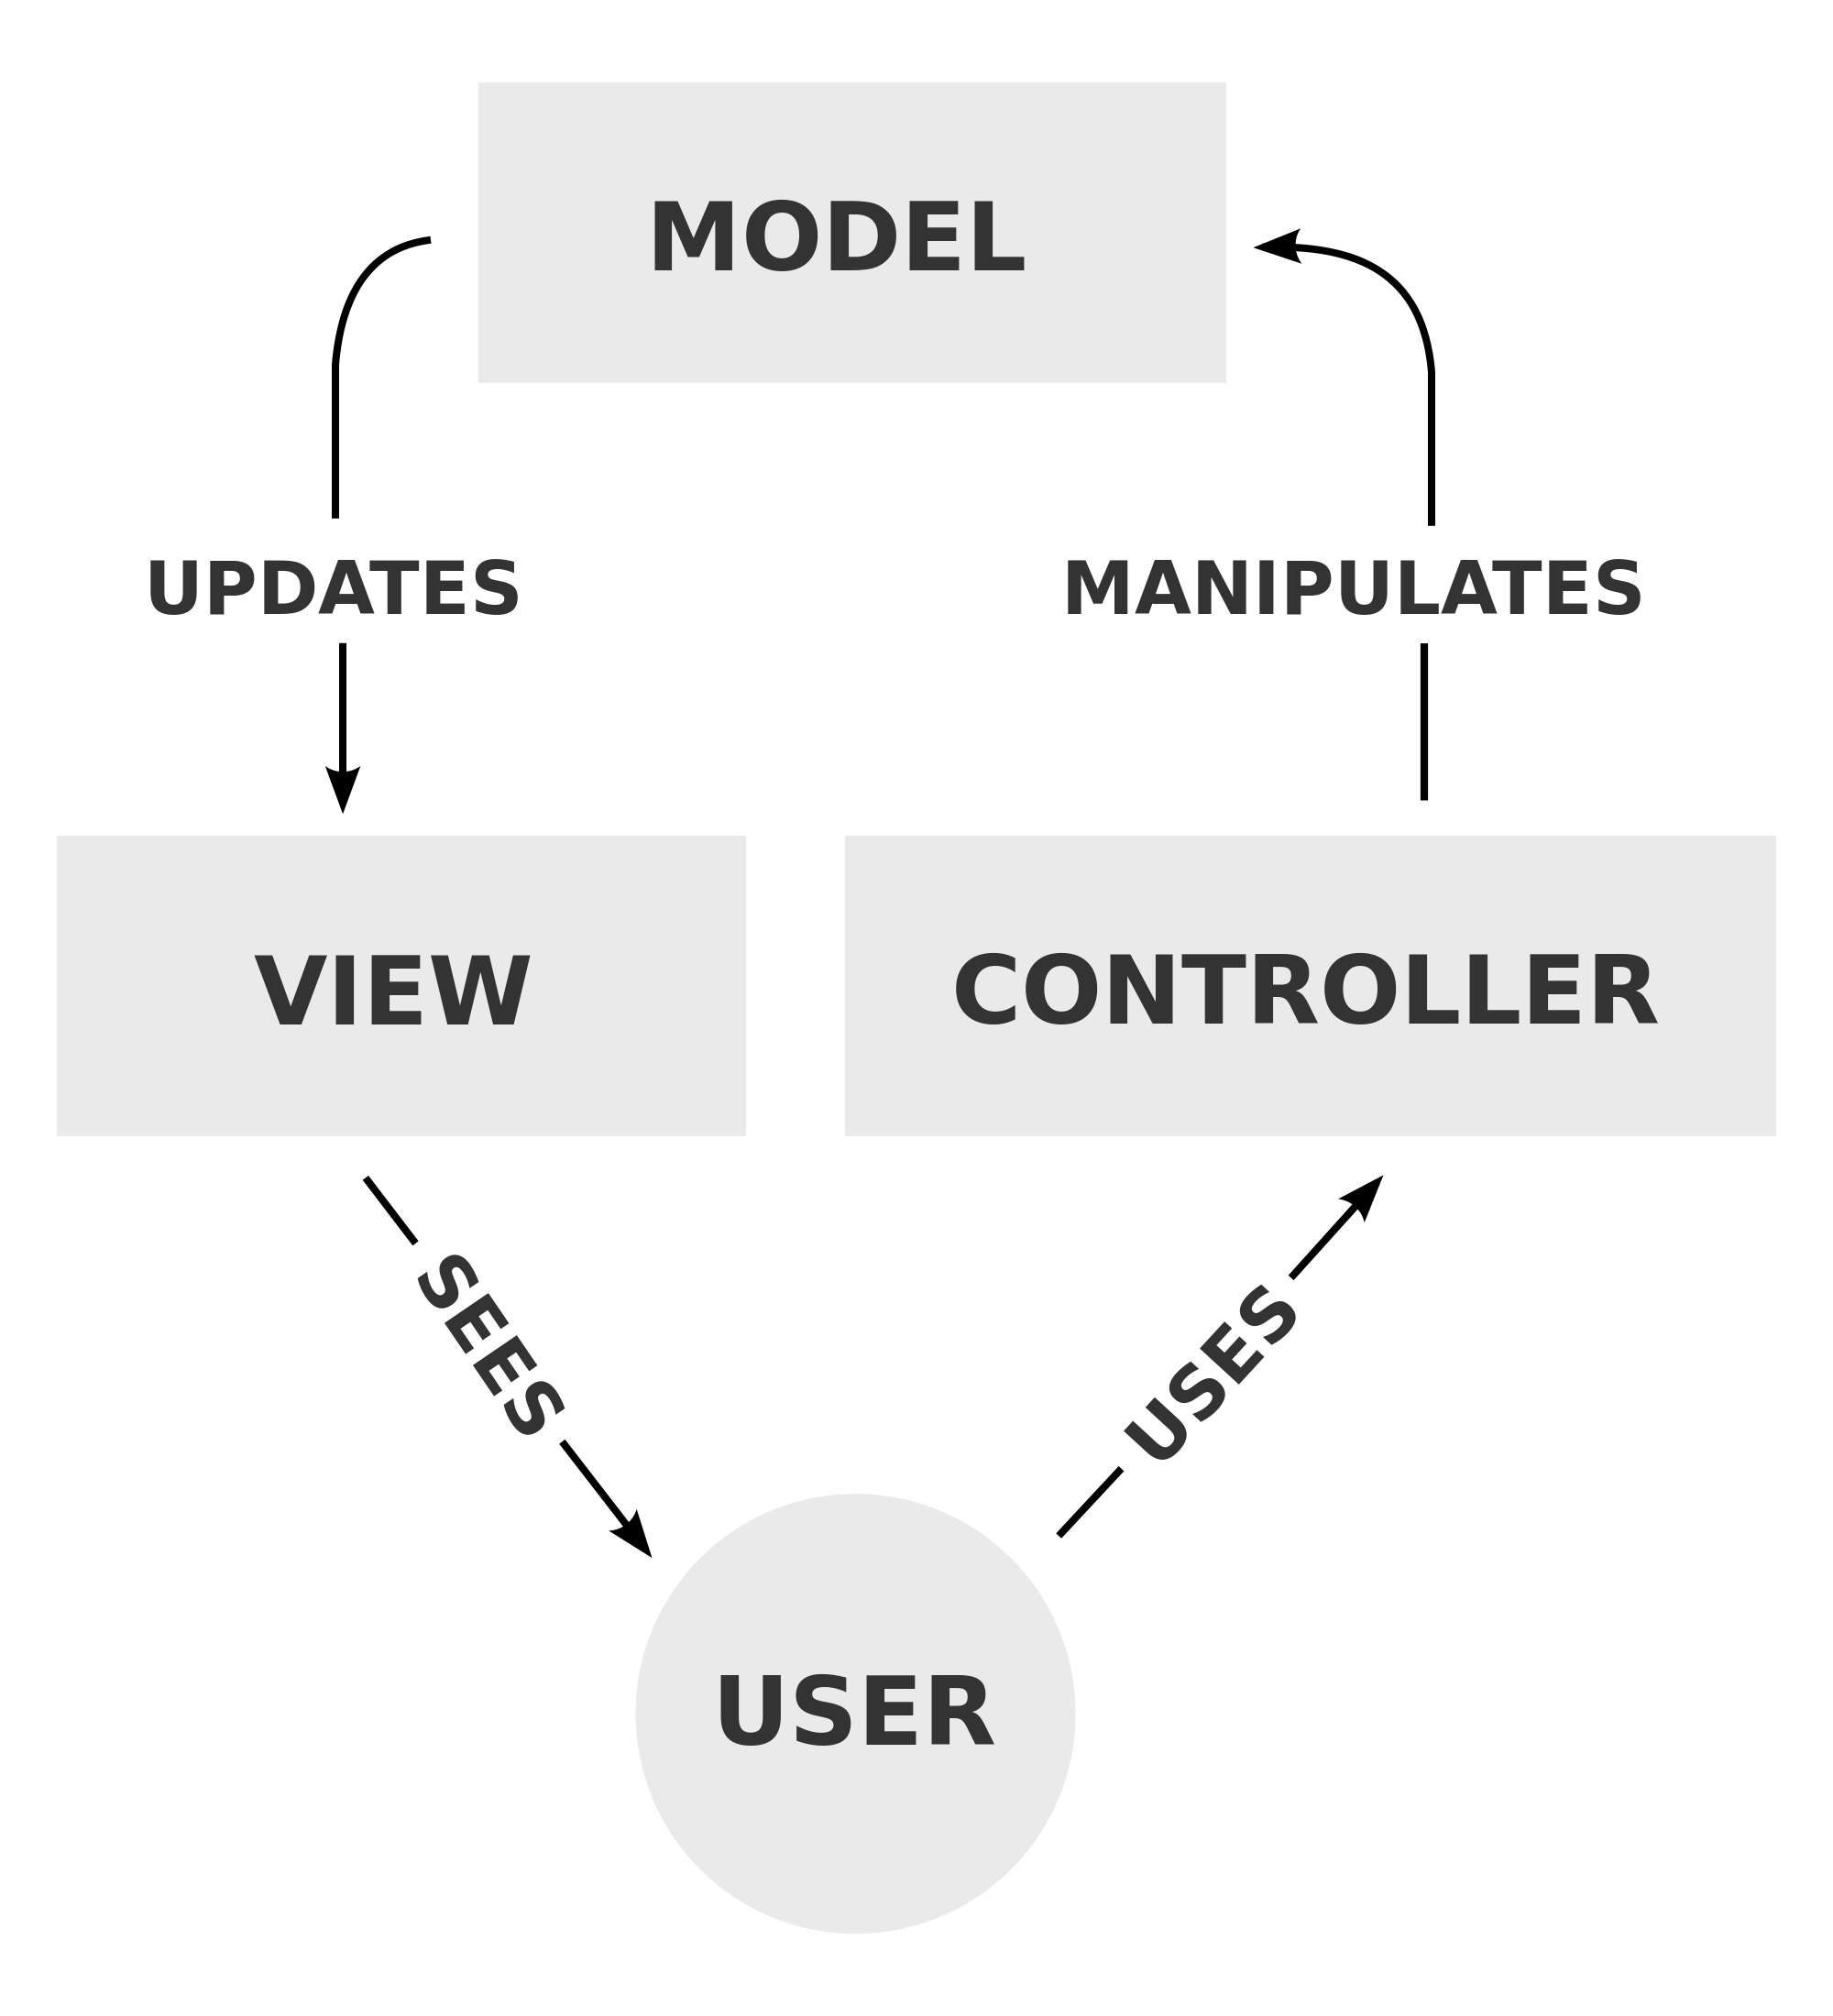
\includegraphics[width=0.5\textwidth]{img/mvc.png}
\end{figure}

\newpage

\section{Spring application}
\subsection{Why Spring instead traditional J2EE?}

\begin{figure}[H]
  \caption{Logo Spring.}
  \centering
    
\includegraphics[width=0.2\textwidth]{img/spring.png}
\end{figure}


Spring is the most popular JAVA framework, It is used in a large parts of professional projects due to its stability, performance and security.
It have a lot of features such as:

\begin{itemize}  
\item Spring provides an easy and secure way to handle forms. With help of DTO for validation, everything is almost automatic.

\item Spring manages the instantiation of the objects without developer worrying about placing instances, when Spring create only one instance and successive calls returns the same object by use of \textit{@Autowired} annotation.

\item Spring is developed in its core with design pattern as Singleton, Factory, MVC... and it is why it is so powerful.
\item Spring is able to manage the dependencies and the configuration of others frameworks.
\end{itemize}  



\subsection{Annotations...}

With Spring and Hibernate, annotations have a very important place in our code, it helps the framework to understand the code and apply special action according to these annotations.
An annotation always begin with the character \textbf{@} and it is placed above a class, a method or an attribute.

\subsubsection{@Autowired}
@Autowired is a Spring specific annotation, It signal to the framework that it have to inject something special at this location.

\begin{figure}[!ht]
  \caption{@Autowired example}
  \centering
    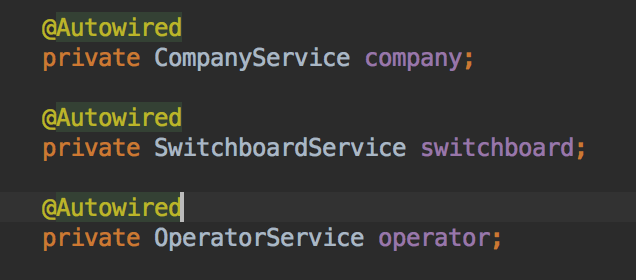
\includegraphics[width=0.7\textwidth]{img/autowired.png}
\end{figure}

In this example, Spring will automatically find the 3 class corresponding to these declarations, and will automatically inject an object and will stock it in cache. So if we call it after again, we will gain performance because it will not be created again.



\section{Application structure}

\subsection{Configuration}
To properly use Spring, we have to let it know which kind of application will be created. Indeed, Spring is a really powerful framework and can be used in lot of different usage.
The configuration of Spring is mainly made by usage of annotations and implementations of some \textit{interfaces}. All following class have to be annotated with \textbf{@Configuration}.\newline

Firstly, we have to tell Spring the application will be a website. According to the official documentation, we have to create a class called \textbf{SpringMvcInitializer} which implements \textit{WebApplicationInitializer}.\newline

Now, Spring knows it will run a website. However, we have to configure some things before it can work properly. We have to create a class \textbf{WebMvcConfig} which extends \textit{WebMvcConfigurerAdapter}. It is in this file, the main settings will be made. For example, it is here we can define the \textbf{view resolver} (we chose Pebble), which will make Spring able to load the views files.  Some others settings will be described in next sections.

\subsection{Login mechanism}

\begin{figure}[H]
  \caption{Login schematic}
  \centering
    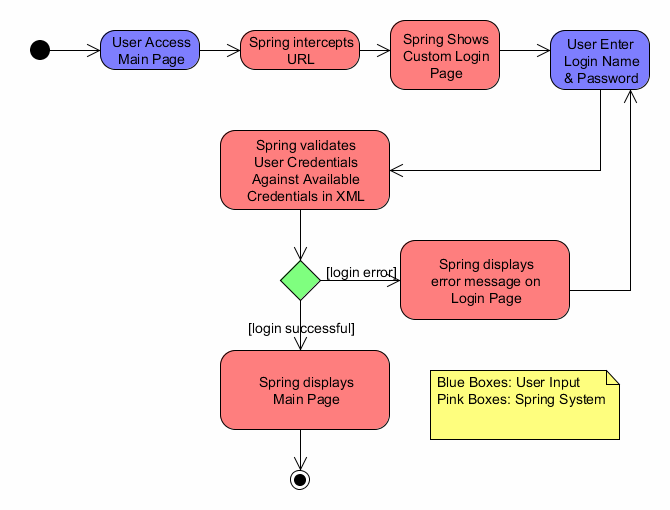
\includegraphics[width=1\textwidth]{img/login.png}
\end{figure}


Here is a schematic representation of a login request processed by Spring, the framework is delivered with its own authentication method in its core. It is why we used this inbuilt system to make our login system. However, its default behaviour doesn't match our requirements. Indeed, by default the login has to be made with an username and a password while we would like to use an email authentication. 

\begin{figure}[H]
  \caption{Login code.}
  \centering
    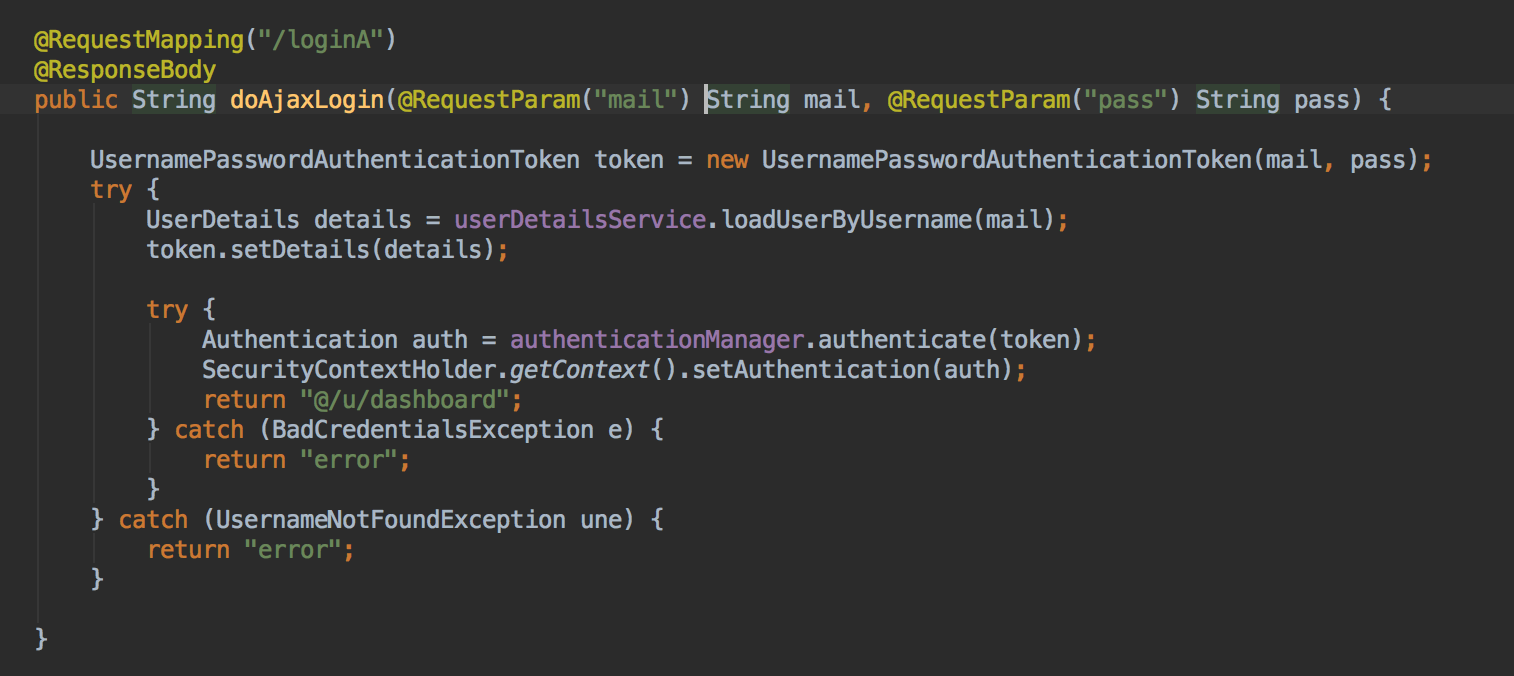
\includegraphics[width=1\textwidth]{img/loginCode.png}
\end{figure}

\subsubsection{User entity, Interface to implement}
To use this login mechanism, we had to implement the interface \textit{UserDetails}. 

\begin{figure}[H]
  \caption{UserDetails interface.}
  \centering
    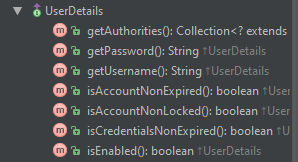
\includegraphics[width=0.7\textwidth]{img/userdetails.png}
\end{figure}

\subsubsection{User service}
As said before, the default behaviour doesn't match our needs. So, we have to create an \textit{UserServiceDetails} which implements the original service interface \textit{UserDetailsService}.

Inside, we have to redefine the method \textit{loadByUsername} to load an user by its email. 

\subsubsection{Security}
For this application, we chose to encrypt password for a better security. Because Spring checks itself if a password is right, we have to tell it how the password is encrypted. This can be done by extending the class \textbf{WebSecurityConfigurerAdapter} and customize the function \textit{configureGlobalSecurity(AuthenticationManagerBuilder auth)}.


\begin{figure}[H]
  \caption{Password encoder.}
  \centering
    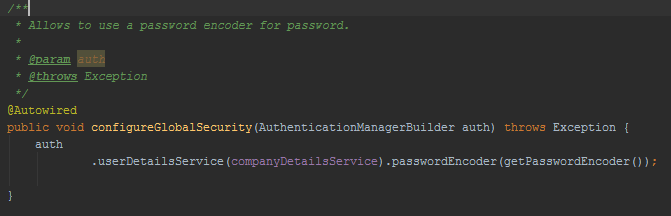
\includegraphics[width=1\textwidth]{img/passwordencoder.png}
\end{figure}





\section{DAO}
\subsection{Controllers}

The controllers are the link between the user and the kernel.
User ask for information : the controller transfer the request to the model, take informations and send them to the view
User give informations : the controller take these informations (after every verifications) and send them to the kernel


\subsection{Hibernate and Models}

The DAO are the link between the program and the database. There are managed by the Hibernate technology, coded in JAVA.
In fact, we have one DAO per entity (switchboard, company...), these files contains functions which returns informations from the database.
\\
\\
Hibernate simplify the interaction with the database, we don't have to use standard SQL interaction.
It works with java object and an hibernate session, we use annotation in the Java class to describe the reproduction of this object in the database,
and we can manipulate this object, transfer it by the session and it will be save on the database.



\begin{figure}[H]
  \caption{Entities relations.
  Full schema in Appendix section.}
  \centering
    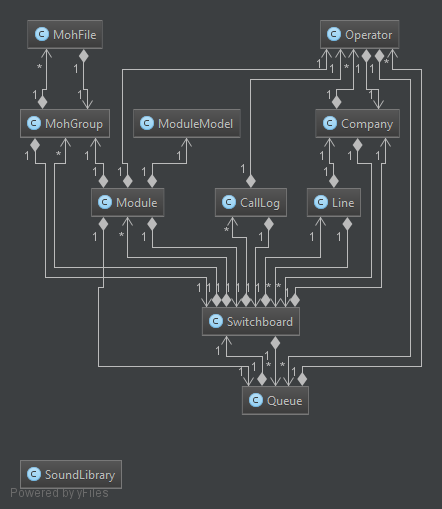
\includegraphics[width=0.7\textwidth]{img/modelsSimple.png}
\end{figure}



\section{Services}

We have an other types of files calls "Services", it works with the DAO files.
Their role are to check data send from the application to the DAO, it's avoid errors in the database.
For example it can check data receive from form.


\subsection{View}

The .twig files are an evolution of the HTML files, there are managed by pebble and represents the view of the website.
A .twig file can represent a file, or a part of a file (a layout), like a that we don't have to code every time the same code (like the menu...)
.twig offer something more than a classical html file, it allow to use Java object inside the view, so we can transfer a list and process it directly inside the view.


\subsection{Converters}

Converters as indicated by his, can convert an object to an other one. Every converters have to implement the interface  \textbf{Converter<S, T>} . The method \textit{convert(S element)} have to return the new object formed with the first one. For example the converter \textit{OperatorIdToOperatorConverter} have for first element an Interger which represent the ID of an operator and it is returned the Operator corresponding. 

\begin{figure}[H]
  \caption{Converters code}
  \centering
    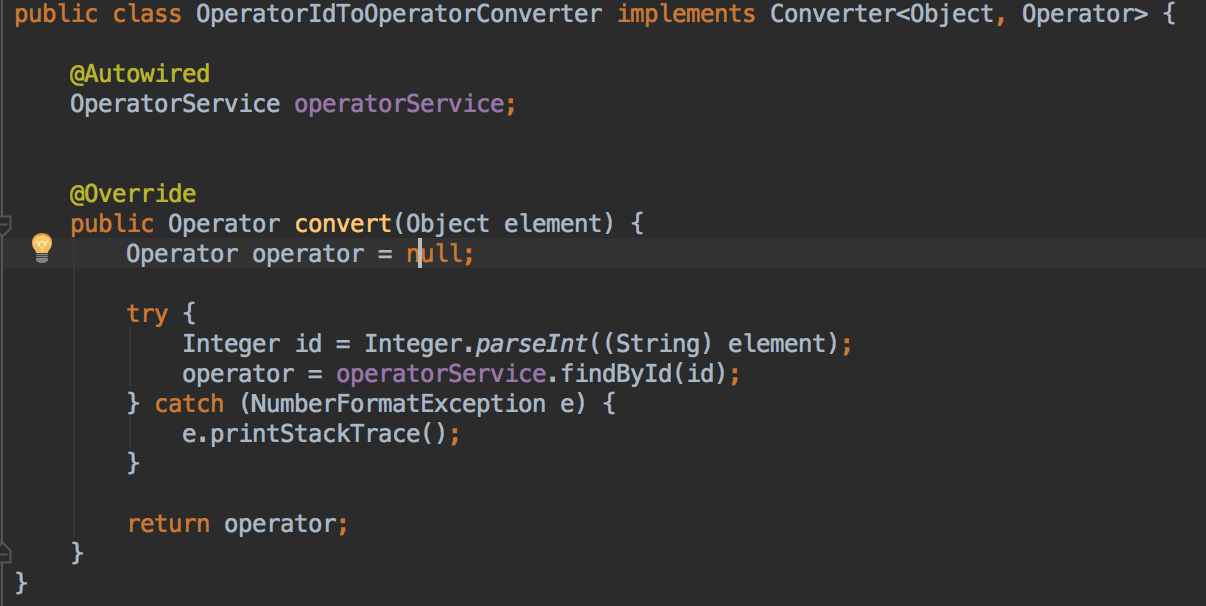
\includegraphics[width=0.8\textwidth]{img/converter.png}
\end{figure}



\subsection{DTO and Validator}

The DTO are a copy of an entity, which explain constraints, for exemple we can say that an attribute should not be longer than 20 characters...
After we put this DTO inside a view in a form, after validation, the DTO will check every constraints, if everything is correct it will send all the data to the controller in one time,
This method allow a gain of time, network ressources and security.

\subsection{Exceptions}

Exceptions are a special type of class which is call only when something goes wrong...
Java provide a large panel of exceptions, we can use them or create our own Exceptions.
The role of the excerptions are to identified quickly when an error occurred, we have a special name for every exceptions so we can know in a few seconds what is going wrong.


\section{Design}
Due to our inability to make a real design, we chose to download a free open-source design. We found the excellent \textit{AdminLTE2} template suitable for a website like our.
\newline

We cleared and adapted it to our website and needs.
This template is based on the Bootstrap framework which ease the front-end development of a website. Furthermore, the Bootstrap framework is a responsive design: it means our website will be functional on every platform (phone, tablets, computer...) and for all screens size.

\begin{figure}[!ht]
  \caption{AdminLTE2.}
  \centering
    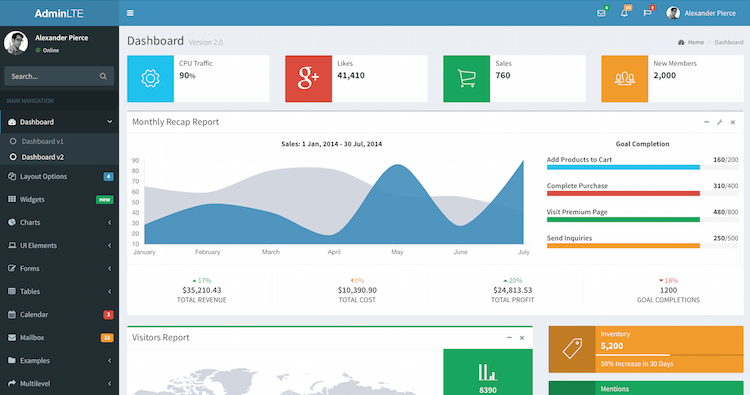
\includegraphics[width=0.9\textwidth]{img/design.png}
\end{figure}





